\documentclass[10pt,twocolumn,letterpaper]{article}

\usepackage{cvpr}
\usepackage{times}
\usepackage{epsfig}
\usepackage{graphicx}
\usepackage{amsmath}
\usepackage{amssymb}
\usepackage{verbatim} % for comment environment
% \usepackage{soul} % for \hl highlighting
% Include other packages here, before hyperref.

% If you comment hyperref and then uncomment it, you should delete
% egpaper.aux before re-running latex.  (Or just hit 'q' on the first latex
% run, let it finish, and you should be clear).
\usepackage[breaklinks=true,bookmarks=false]{hyperref}

\cvprfinalcopy % *** Uncomment this line for the final submission

\def\cvprPaperID{****} % *** Enter the CVPR Paper ID here
\def\httilde{\mbox{\tt\raisebox{-.5ex}{\symbol{126}}}}

% Pages are numbered in submission mode, and unnumbered in camera-ready
%\ifcvprfinal\pagestyle{empty}\fi
%\setcounter{page}{4321}
%\DeclareMathSymbol{\Tangent}
\begin{document}
\title{Unmentioned approximations in Dense CRF}
\author{Vikas Dhiman\\
{\tt\small vdhiman@nec-labs.com}
}
\maketitle
\begin{abstract}
  Fully connected CRF like those presented in \cite{krahenbuhl2012efficient}
  use some approximations that are neither mentioned nor justified in the
  paper.
\end{abstract}

% What is a random field? A graphical representation defining the probabilistic
% interdependencies among different random variables. When you are modeling
% something as dense CRF, you are basically claiming that every variable is
% dependent on each other.
% 
% The pairwise Gibbs energy claimed in 
% \cite[Eq(1)]{krahenbuhl2012efficient} is not a Gibbs energy because it is not defined
% on cliques rather than pair of variables. The term used \emph{fully connected
% pairwise CRF model} is itself contradictory because the CRF if fully connected
% cannot be pairwise.
% 
% As far as I can understand the authors have not presented or referred to any
% results as to why the \emph{dense CRF} can be factorized into pairwise
% energies.
% 
% If higher order graphical models were representable as pairwise energies,
% there would have been no problem in inferring on them.
\section{Dense CRF}

% \subsection{Correct factorization of a dense CRF}
By Hammersley Clifford theorem, there exists a factorization of a graphical
model such that total probability of any part of the graph can be written as
product of positive functions of its cliques
\cite[145]{grimmett2010probability}. Writing the factorization domain, the
energy of dense CRF should be 
\begin{multline}
  E(\mathbf{x}) = \sum_i \psi_u(x_i) + \sum_{i < j} \psi_p(x_i, x_j)\\
  + \sum_{i < j < k} \psi_t(x_i, x_j, x_k)
  + \dots
  + \psi(\mathbf{x})
\end{multline}

This does not help because we get a term $\psi_{\mathbf{x}}$ that is as big as
$E(\mathbf{x})$. This shows that dense CRFs are anti-thesis of CRF which are
meant to define sparse interdependencies between variables so that probability
over large number of random variables can be factorized into smaller
tractable problems using domain knowledge. Without using factorizable CRF, the
authors have not used any of the useful theorems that have been established in
the field of graphical models.

However, the authors in \cite{krahenbuhl2012efficient} invent a new term
called \emph{fully connected pairwise CRF model} and without any explanation 
introduce the following energy function.

\begin{align}
  E(\mathbf{x}) = \sum_i \psi_u(x_i) + \sum_{i < j} \psi_p(x_i, x_j)
\end{align}

Clearly this is a linear approximation of energy function. The energy function
is assumed to weighted sum of pairwise energies over different variable
states. How well the energy function can be approximated depends on the energy
function itself. For comparison we present \ref{fig:compare} a 2D Gaussian compared with an
approximation of Gaussian that is generated by sum of two 1D Gaussians.
\begin{figure}
  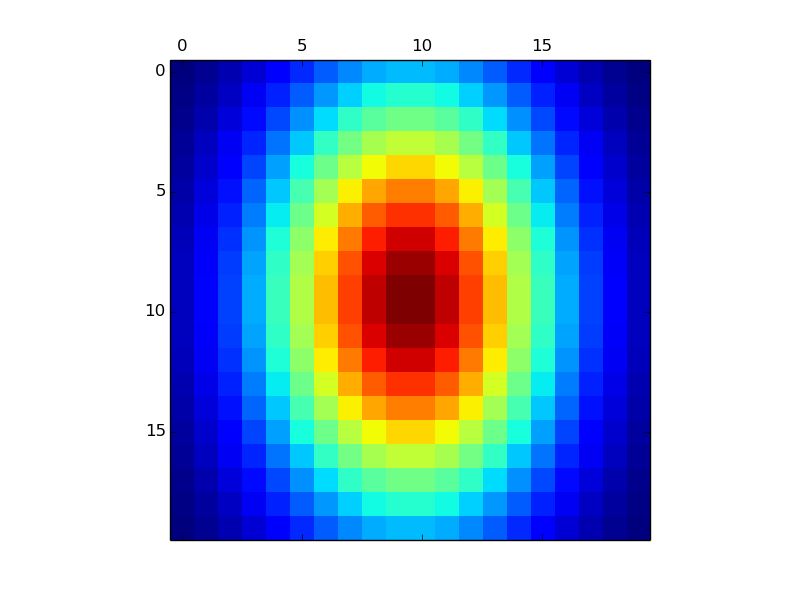
\includegraphics[width=0.5\columnwidth]{graphics/gaussian2D.png}%
  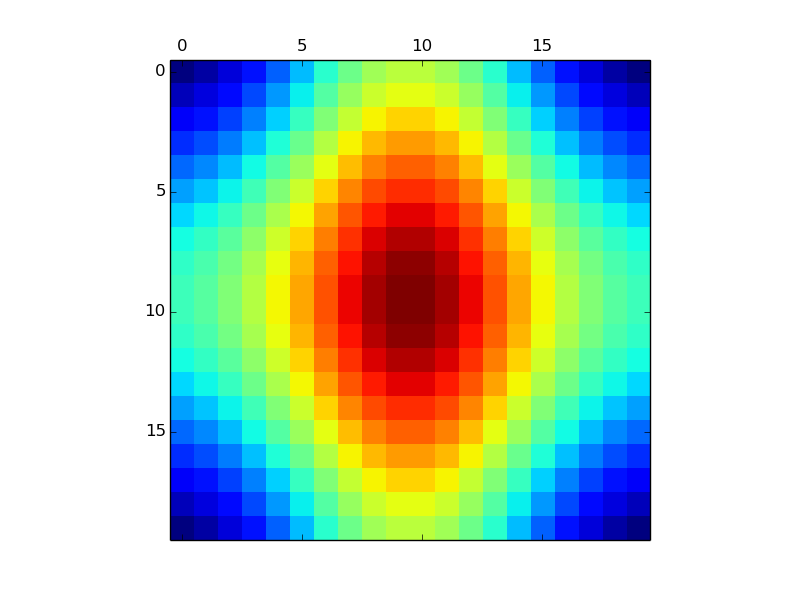
\includegraphics[width=0.5\columnwidth]{graphics/gaussianLinear1D.png}%
  \caption{Comparison of a 2D Gaussian (left) compared with an
    approximation of Gaussian (right) that is generated by sum of two 1D
  Gaussians.}
  \label{fig:compare}
\end{figure}

Intuitively, the approximation of a 2D Gaussian using sum of 1D Gaussians is
like approximating 2D Euclidean distance by using linear combination of 1D
distance only which is commonly known as L1 or manhattan distance. Note that
the deviation of approximation is minimal around the center of the Gaussian
and around the axes and becomes more prominent as the distance increases.

There are a few open questions here:
\begin{enumerate}
  \item How good is this approximation?  What are the error bounds of the
approximation? Can I check an energy function for error bounds?
\item Is this better than the sparse CRFs? (at least in gaussian kernel pairwise
energies)
\item What lessons can we take from empirical success of dense CRFs and how can
we make sparse CRFs better or vice versa?
  
\end{enumerate}


% In the dense CRF paper, the authors constrain the energy over the graph to be
% only pairwise energy. The pairwise energies are modeled in the paper as
% Gaussian distance between the feature vectors and positions of the points.
% However, if we consider higher order terms the energies could have been more
% complex 

{\small
\bibliographystyle{ieee}
\bibliography{densecrf}
}

\end{document}
